\documentclass[11pt,a4paper]{letter}
\usepackage[top=0.50in, bottom=0.5in, left=1.1in, right=1.1in]{geometry}
\usepackage{graphicx}

%\signature{}

\usepackage{Sweave}
\begin{document}

\begin{letter}{}

\includegraphics[width=0.3\textwidth]{logo_uah.png}

\opening{Dear Dr. Wake:}

\noindent Please consider our paper, entitled `Phylogenetic estimates of species-level phenology improve ecological forecasting' as a Letter in \emph{Nature Climate Change.} 
\vspace{1.5ex}\\
Accurately predicting the impacts of climate change on key ecosystem services is a major challenge to tailor effective mitigation and adaptation strategies. Yet, ecological forecasting of underlying processes such as plant phenology, is trapped by relying on data for few species, which often leads to predictions that fail at capturing the high variability observed across the responses of different species.
\vspace{1.5ex}\\
Current hierarchical models (e.g. HMM) have increased their popularity as they can deal with issues related to some species being more data-abundant than others. These models allow inference across species by pooling estimations of data-poor species towards those of more prevalent ones assuming that all species are equivalent. Quite the contrary, species are nested within lineages whose phenological responses to cues have followed particular evolutionary trajectories. Thus, if the model estimates for a data-poor species are assimilated to average estimations of data-rich species from a distant lineage with complete different phenological behavior, large biases can arise.
\vspace{1.5ex}\\
We propose an approach that extends the Phylogenetic Mixed Model by allowing phylogenetic structure to inform species-level sensitivities to cues, to tackle mentioned biases. Here, we demonstrate the superior performance of a new formulation for Phylogenetic Mixed Models compared to commonly used Hierarchical Mixed Models. Our results show that, (1) variability across species is larger than variability across cues, (2) PMM formulations outperform HMM, particularly for data deficient species and (3) Phylogenetic modelling formulations such as ours informs how different clades have evolved their phenotypes in response to multiple environmental cues operating jointly. The findings presented in this study have significant implications for improving ecological forecasting under scenarios of changing climate.
\vspace{1.5ex}\\
The potential impact of our findings on ecological forecasting are not restricted to predictions of phenology. Instead, Phylogenetic Mixed Models such as ours could (and should) be applied to other phenotypic traits that may have been configured in response to multiple drivers, differently so for different lineages. This is particularly relevant in a context where forecasts of functional responses of organisms in response to accelerating warming are urged to safeguard the provision of ecosystem services.
\vspace{1.5ex}\\
We have suggested three possible reviewers (see online submission system: {\bf XX, XX2, XX3}). We believe that our manuscript aligns well with the scope and objectives of \emph{Nature Climate Change}. It is not under consideration elsewhere. We hope that you will find it suitable for publication, and look forward to hearing from you.
\vspace{1.5ex}\\
\noindent Sincerely,\\
\vspace{1.5ex}\\
 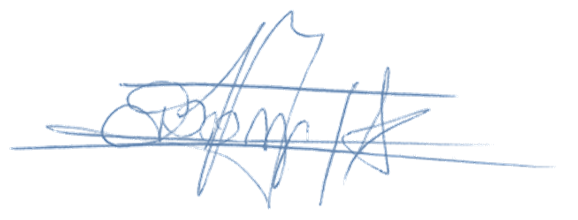
\includegraphics[width=0.2\textwidth]{Signature_IMC.png} \\
 \vspace{1.5ex}\\
\noindent Ignacio Morales-Castilla


\end{letter}
\end{document}
